\message{ !name(main.tex)}\documentclass{article}

\PassOptionsToPackage{numbers, compress}{natbib}





\usepackage[final]{neurips_2022}









\usepackage[utf8]{inputenc} \usepackage[T1]{fontenc}    \usepackage{hyperref}       \usepackage{url}            \usepackage{booktabs}       \usepackage{amsfonts}       \usepackage{nicefrac}       \usepackage{microtype}      \usepackage[dvipsnames]{xcolor}
\usepackage{colortbl,booktabs}
\usepackage{environ}
\usepackage{multicol}
\usepackage{multirow}
\usepackage{amsthm}
\usepackage{graphicx}
\usepackage{tikz}
\usepackage{amsmath}
\usepackage{wrapfig}
\usepackage{makecell}
\usepackage{diagbox}
\usepackage{pifont}
\usepackage{diagbox}
\usepackage[noend]{algpseudocode}
\usepackage{algorithm2e}
\RestyleAlgo{ruled}
\NewEnviron{elaboration}{
	\par
	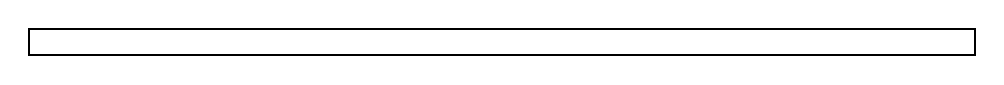
\begin{tikzpicture}
		\node[rectangle,minimum width=0.99\textwidth] (m) {\begin{minipage}{0.99\textwidth}\BODY\end{minipage}};
		\draw[thick] (m.south west) rectangle (m.north east);
	\end{tikzpicture}
}

\PassOptionsToPackage{hyphens}{url}
\hypersetup{colorlinks=true}

\definecolor{Tianlong_color}{rgb}{0.858, 0.188, 0.478}
\newcommand{\TL}[1]{\textcolor{Tianlong_color}{TL: #1}}

\newcommand{\Add}[1]{\textcolor{blue}{#1}}

\def\mE{\mathbb{E}}
\def\mR{\mathbb{R}}
\def\bx{{\bf x}_i}
\def\bX{{\bf X}}
\def\cx{{\bf x}_{(k)}}
\def\tilx{\tilde{\bf x}_i}
\def\tilX{\tilde{\bf X}}
\def\std{std}
\def\bU{{\bf U}}

\newcommand{\bm}[1]{\mathbf{#1}}

\title{A Comprehensive Study on Large-Scale Graph Training: Benchmarking and Rethinking}



\author{Keyu Duan\textsuperscript{1}, Zirui Liu\textsuperscript{2}, Peihao Wang\textsuperscript{3}, Wenqing Zheng\textsuperscript{3}, \\ \textbf{Kaixiong Zhou\textsuperscript{2}, Tianlong Chen\textsuperscript{3}, Xia Hu\textsuperscript{2}, Zhangyang  Wang\textsuperscript{3}} \\
\textsuperscript{1}National University of Singapore, \textsuperscript{2}Rice University, \textsuperscript{3}University of Texas at Austin \\
    \small{\texttt{\{k.duan\}@u.nus.edu;}}
	\small{\texttt{\{zl105,Kaixiong.Zhou,xia.hu\}@rice.edu;}}  \\
	\small{\texttt{\{peihaowang,w.zheng,tianlong.chen,atlaswang\}@utexas.edu}}
}

\begin{document}

\message{ !name(main.tex) !offset(-3) }


\maketitle
\vspace{-5mm}
\begin{abstract}
	Large-scale graph training is a notoriously challenging problem for graph neural networks (GNNs). Due to the nature of evolving graph structures into the training process, vanilla GNNs usually fail to scale up, limited by the GPU memory space. Up to now, though numerous scalable GNN architectures have been proposed, we still lack a comprehensive survey and fair benchmark of this reservoir to find the rationale for designing scalable GNNs. To this end, we first systematically formulate the representative methods of large-scale graph training into several branches and further establish a fair and consistent benchmark for them by a greedy hyperparameter searching. In addition, regarding \textit{efficiency}, we theoretically evaluate the time and space complexity of various branches and empirically compare them w.r.t GPU memory usage, throughput, and convergence. Furthermore, We analyze the pros and cons for various branches of scalable GNNs and then present a new ensembling training manner, named \textit{EnGCN}, to address the existing issues. Remarkably, our proposed method has achieved new state-of-the-art (SOTA) performance on large-scale datasets. Our code is available at \url{https://github.com/VITA-Group/Large_Scale_GCN_Benchmarking}.
\end{abstract}

\section{Introduction}
\vspace{-2mm}
The Graph Neural Networks (GNNs) have shown great prosperity in recent years~\citep{kipf2016semi,velickovic2017graph,hamilton2017inductive,xu2018powerful}, and have dominated a variety of applications, including recommender systems~\citep{he2020lightgcn,ying2018graph,zheng2021cold}, social network analysis~\citep{tang2009relational,gao2018large,huang2019graph}, scientific topological structure prediction (e.g. cellular function prediction~\citep{hu2020open,zitnik2017predicting}, molecular structure prediction~\citep{hu2019strategies,you2020graph}, and chemical compound retrieval~\citep{wale2008comparison}), and scalable point cloud segmentation~\citep{li2019deepgcns,wang2019dynamic}, etc. Although the message passing (MP) strategy provides GNNs' superior performance, the nature of evolving massive topological structures prevents MP-based GNNs~\citep{li2020deepergcn,klicpera2018predict,xu2018representation,kipf2016semi,velickovic2017graph,xu2018powerful,gao2019graph, zhou2019multi} from scaling to industrial-grade graph applications. Specifically, as MP requires nodes aggregating information from their neighbors, the integral graph structures are inevitably preserved during forward and backward propagation, thus occupying considerable running memory and time. For example~\citep{ying2018graph}, training a GNN-based recommendation system over 7.5 billion items requires three days on a 16-GPU cluster (384 GB memory in total).

To facilitate understanding, a unified formulation of MP with  layers is presented as follows:

where  is an activation function (e.g. ReLU) and  is the weighted adjacency matrix at the -th layer. As in Equ.~\eqref{equ:message_passing}, the key bottleneck of vanilla MP lies on . For the memory usage, the entire sparse adjacency matrix is supposed to be stored in one GPU. As the number of nodes grows, it is quite challenging for a single GPU to afford the message passing over the full graph.

Up to now, massive efforts have been made to mitigate the aforementioned issue and scale up GNNs~\citep{chiang2019cluster, zeng2019graphsaint, hamilton2017inductive, chen2018fastgcn, zou2019layer, wu2019simplifying, frasca2020sign, sun2021scalable, zhang2021graph}. Most of them focus on approximating the iterative full-batch MP to reduce the memory consumption for training within one single GPU. It is worth noting that we target at the algorithmic scope and do not extend to scalable infrastructure topics like distributed training with multiple GPUs~\citep{bojchevski2020scaling,md2021distgnn} and quantization~\citep{liu2021exact}. Briefly, the previous works encompass two branches: \textit{Sampling-based} and \textit{Decoupling-based}. Namely, the former methods~\citep{hamilton2017inductive, chen2018fastgcn, zeng2019graphsaint, chiang2019cluster, chen2017stochastic, cong2020minimal, huang2018adaptive} perform \textit{batch training} that utilizes sampled
subgraphs as a small batch to approximate the full-batch MP so that the memory consumption is considerably reduced. The latter follows the principle of performing \textit{propagation} ( and \textit{prediction} ( separately, either precomputing the propagation~\citep{wu2019simplifying, frasca2020sign, klicpera2018predict, liu2022neighbor2seq, bojchevski2020scaling} or post-processing with label propagation~\citep{sun2021scalable, huang2020combining}. Despite the prosperity of scalable GNNs, there are still plights under-explored:
we lack a systematic study of the reservoir from the perspective of \textit{effectiveness} and \textit{efficiency}, without which it is unachievable to tell the rationale of the designing philosophy for large-scale graph learning in practice.

To this end, we first establish a consistent benchmark and provide a systematic study for large-scale graph training for both \textit{Sampling-based} methods~(Sec.~\ref{sec:formu_sampling}) and \textit{Decoupling-based} methods~(Sec.~\ref{sec:formu_decoupling}). For each branch, we conduct a thorough investigation of the design strategy and implementation details of typical methods. Then, we carefully examine the sensitive hyperparameters and unify them in one ``sweet spot'' set by a linear greedy hyperparameter (HP) search (Sec.~\ref{sec:benchmarking_effectiveness}), i.e., iteratively searching the optimal value for an HP while fixing the others. For all concerned methods, the performance comparison is conducted on representative datasets of different scales, varying from about  nodes to , including Flickr~\citep{zeng2019graphsaint}, Reddit~\citep{hamilton2017inductive}, and ogbn-products~\citep{hu2020open}. This step is a crucial precondition on our way to the ultimate as the configuration inconsistency significantly prohibits a fair comparison as well as the following analysis. Besides, regarding \textit{efficiency}, we theoretically present the time and space complexities for the various branches, and empirically evaluate them on GPU memory usage, throughput, and convergence (Sec.~\ref{sec:benchmarking_efficiency}). In addition to the benchmark, we further present a new ensembling training manner \textit{EnGCN} (Sec.~\ref{sec:engcn}) to address the existing issues mentioned in our benchmark analysis (Sec.~\ref{sec:pros_and_cons}). Notably, via organically integrating with self-label-enhancement (SLE)~\cite{sun2021scalable}, EnGCN achieves the new state-of-the-art (SOTA) on multiple large-scale datasets.

\vspace{-1mm}
\section{Formulations For Large-scale Graph Training Paradigms}\label{sec:formulation}
\vspace{-2mm}
\subsection{Sampling-based Methods}\label{sec:formu_sampling}
\vspace{-2mm}
Given the formulation of Equ.~\eqref{equ:message_passing}, \textit{sampling-based} paradigm seeks the optimal way to perform batch training, such that each batch will meet the memory constraint of a single GPU for message passing. For completeness, we restate the unified formulation of sampling-based methods as follows:

where  is the set of sampled nodes for the -th layer, and  is the adjacency matrix for the -th layer sampled from the full graph. Given the local view of GNN --- one node's representation is only related to its neighbors --- a straightforward way for unbiased batch training would be , where  denotes the set of neighbors.  is randomly sampled according to the uniform distribution. Notably, this batch training style could achieve SOTA performance but also suffers from the ``\textit{neighbor explosion}'' problem, where the time consumption and memory usage grow exponentially with the GNN depth, causing significant memory and time overhead. To mitigate this, a number of \textit{sampling-based} methods were proposed. The key difference among them is how  are sampled. Given a large-scale graph , there are three categories of widely-used sampling strategies:

\vspace{-2mm}
\paragraph{Node-wise Sampling~\cite{hamilton2017inductive}}\label{sec:node_wise_sampling.}
, where  is a sampling distribution;  is the sampling space, i.e., the -hop neighbors of ; and  denotes the number of samples. The representative node-wise sampling method is:

 \textit{GraphSAGE}~\citep{hamilton2017inductive}: In GraphSAGE,  is the uniform distribution.

Compared with the aforementioned \textit{naive batch training}, the node-wise sampling~\citep{hamilton2017inductive} alleviates the "\textit{node explosion}" problem by fixing the number of sampled neighbors  for each node. It thus reduces the space complexity from  to , where  is the averaged node degree. However, as  is not far less than  in order of magnitude, such mitigation is moderate, which is empirically validated by our empirical results in Sec.~\ref{sec:benchmarking_effectiveness} and Sec.~\ref{sec:benchmarking_efficiency}.

\vspace{-2mm}
\paragraph{Layer-wise Sampling~\cite{chen2018fastgcn,zou2019layer}.}\label{sec:layer_wise_sampling}
, where  denotes the union of -hop neighbors of all nodes in .  We introduce a couple of layer-wise sampling methods as follows.

 \textit{FastGCN}~\citep{chen2018fastgcn}: The sampling distribution  is designed regarding the node degree, where the probability for node  of being sampled is .

 \textit{LADIES}~\citep{zou2019layer}: More recently, based on FastGCN, Zou et.al.~\citep{zou2019layer} propose LADIES that extends the sampling space from  to  by adding the self-loops.

Notably, Compared with the node-wise sampling, the layer-wise sampling essentially solves the ``\textit{neighbor explosion}'' problem by fixing the number of overall sampled nodes in a layer to . However, the layer-wisely induced adjacency matrix is usually sparser than the others, which accounts for its sub-optimal performance in practice.

\vspace{-2mm}
\paragraph{Subgraph-wise Sampling~\cite{chiang2019cluster,zeng2019graphsaint}.}\label{sec:subgraph_wise_sampling}
 In the subgraph-wise sampling, all layers share the same subgraph induced from the entire graph  based on a specific sampling strategy , such that the sampled nodes are confined in the subgraph. Typically, this sampling strategy has two representative works:

~\textit{ClusterGCN}~\citep{chiang2019cluster}: ClusterGCN first partitions the entire graph into clusters based on some graph partition algorithms, e.g. METIS~\citep{karypis1998fast}, and then select several clusters to form a batch.

~\textit{GraphSAINT}~\citep{zeng2019graphsaint}: GraphSAINT samples a subset of nodes based on sampling strategy  and then induces the corresponding subgraph as a batch. The commonly-used sampling strategies include:  node sampler: ,  edge sampler: , and  random walk sampler. They are illustrated in Appendix~\ref{app:sampling_schemes}.

\vspace{-2mm}
\subsection{Decoupling-based Methods}\label{sec:formu_decoupling}
\vspace{-2mm}
Training GNNs with full-batch message passing at each epoch is not plausible. In this section, we summarize another line of scalable GNNs which decouple the message passing from GPU training to CPUs. Specifically, the message passing is conducted only once at CPUs accompanied by large accessible memory. Depending on the processing order, there are two typical ways to decouple these two operations:  \textit{pre-processing} and  \textit{post-processing}.

\vspace{-2mm}
\paragraph{Pre-processing: MP precomputating~\cite{wu2019simplifying,frasca2020sign,sun2021scalable}.} Recalling Equ.~\eqref{equ:message_passing}, without loss of generalization, we assume that , i.e. the topological structure for the entire graph remains the same during forward propagation, meeting most of the cases. To decouple the two operations, \textit{message passing} () and \textit{feature transformation} (), we can first pre-compute the propagated node representations and then train a neural network for the downstream task based on these fused representations:

where  can be regarded as the node representation aggregating -hop neighborhood information;  is the largest propagation hop;  is a function that combines the aggregated features from different hops; and  is a feature mapping function parameterized by . We summarize three existing pre-computing schemes as follows.

 \textit{SGC}~\cite{wu2019simplifying}: SGC leverages the node representations aggregated with k hops and feeds the resultant features to a full-connected layer. We can formulate this scheme by letting  select the last element  and  be a linear layer with readout activation: .

\noindent
 \textit{SIGN}~\cite{frasca2020sign}: SIGN concatenates features from different hops and then fuse them as the final node representation via a linear layer. To be more specific,  is defined as , where  is a transformation matrix, and  is defined as a linear readout layer .

\noindent
 \textit{SAGN}~\cite{sun2021scalable}: SAGN adopts attention mechanism to combine feature representations from  hops: , where  is a diagonal matrix whose diagonal corresponds to the attention weight for each node of -hop information. The attention weight for the -th node is calculated by , where the subscripts slices the data matrices along the row.
The feature mapping function is implemented by an MLP block with a skip connection to initial features: .


\vspace{-2mm}
\paragraph{Post-processing: Label Propagation.}
The label propagation algorithms~\citep{zhu2005semi, wang2007label, karasuyama2013manifold, gong2016label, liu2018learning, huang2020combining, wang2020unifying} diffuse labels in the graph and make predictions based on the diffused labels. It is a classical family of graph algorithms for \textit{transductive learning}, where the nodes for testing are used in the training procedure. The label propagation can be written in a unified form as follows:

The diffusion procedure iterates the formula above with  for multiple times to guarantee convergence. It requires two sets of inputs:  the stack of the \textit{label embeddings} of all nodes, denoted as , where  is the number of classes. In our implementation, the  is the output of a trained MLP model~\cite{huang2020combining}.  the \textit{diffusion embedding}, denoted as  that propagate themselves across the edges in the graph. Depending on how the diffusion embeddings of unlabeled nodes are computed, two types of  are summarized as follows:



 \textit{Zeros}~\citep{zhu2005semi}:
, where  denotes the training set and  is the stack of true labels. For \textit{zeros}, .

 \textit{Residual}~\citep{huang2020combining}:
, where .  is the predictions of a trained simple neural network, e.g. MLP, and  is an residual error matrix, which is optimized iteratively for multiple times by , where  and .

\vspace{-2mm}
\subsection{More Related Works}
\vspace{-2mm}
\textbf{Model-agnostic Tricks.} Besides the training methods as introduced above, there are some model-agnostic tricks that have been empirically confirmed to be effective for boosting large-scale graph training. Although those add-ons cannot be included into our benchmarking analysis, it is of equal importance to introduce them for completeness. Here we briefly introduce two representative ones:

 \textit{Self-Label-Enhanced (SLE)}~\cite{sun2021scalable}: SLE includes two individual tricks, \textit{self training} and \textit{label augmentation}. Here we use  denoting the training set. For self training, the unlabeled nodes with high confidence (larger than a pre-defined threshold) are added to  after a certain number of training epochs. For label augmentation, it trains an additional model . The forward propagation can be formulated as .  is added to the main model to make the final prediction.

 \textit{GIANT}~\cite{chien2021node}: In general, node features are usually pre-embed with graph-agnostic language models, such as word2vec~\cite{mikolov2013distributed} and BERT~\cite{devlin2018bert}. Recently, Chien et.al. propose a graph-related node feature extraction framework (GIANT), which embeds the raw texts to numerical features by taking advantage of graph structures, to help boost the performance of GNNs for the downstream tasks.

\textbf{Memory-based GNN Training}. Focus on mitigating the ``\textit{Neighbor Explosion}'' problem of full-batch training as introduced, memory-based GNNs~\cite{fey2021gnnautoscale, ding2021vq} try to save the GPU memory with different techniques while including all neighbor nodes into computing during the message passing. GAS~\cite{fey2021gnnautoscale} incorporates \textit{historical embeddings}~\cite{chen2017stochastic} to provably maintain the expressive power of full-batch GNN. VQ-GNN~\cite{ding2021vq} utilizes \textit{vector quantization} to scale convolutional-based GNN and resemble the performance of full-batch message passing by learning an additional quantized feature matrix and a corresponding low-rank adjacent matrix.

\vspace{-3mm}
\section{Benchmarking Over Effectiveness}\label{sec:benchmarking_effectiveness}
\vspace{-1mm}
\subsection{Implementation Details}
\vspace{-1mm}
We test numerous large-scale graph training methods with a greedy hyperparameter (HP) search to find their \textit{sweet spot} and the best performance for a fair comparison. The search space is defined in Table~\ref{tab:search_space}. The access and statistics of all used datasets are introduced in Appendix~\ref{app:datasets}. Particularly, for label propagation, we select two representative algorithms: Huang et.al.~\citep{huang2020combining}, the \textit{residual} diffusion type, and Zhu et.al.~\citep{zhu2005semi}, the \textit{zeros} type. The number of propagation is the maximum iteration . The aggregation ratio is  as in Equ.~\eqref{equ:lp}, and the number of MLP layers is the number of MLP layers that precedes the label propagation module following Huang et.al.~\citep{huang2020combining}.
\begin{wraptable}{r}{0.55\linewidth}
	\vspace{-3mm}
	\caption{The search space of hyperparameters for benchmarked methods.}
	\label{tab:search_space}
	\centering
	\resizebox{1\linewidth}{!}{
		\begin{tabular}{cl|c}
			\toprule
			Category            & Hyperparameter (Abbr.)   & Candidates                                                                             \\
			\midrule
			\multirow{7}{*}{\shortstack{Sampling \&                                                                                                 \\ Precomputing}} & Learning rate (LR) &    \\
			                    & Weight Decay (WD)        &                                                              \\
			                    & Dropout Rate (DP)        &                                                            \\
			                    & Training Epochs (\#E)    &                                                                \\
			                    & Hidden Dimension (HD)    &                                                                     \\
			                    & \# layers (\#L)          &                                                                     \\
			                    & Batch size (BS)      &                                                              \\
			\midrule
			\multirow{6}{*}{LP} & Diffusion Type (DT)      & \{ residual, zeros \}                                                              \\
			                    & \# Propagations (\#Prop) & \{ 2, 20, 50 \}                                                                    \\
			                    & Aggregation Ratio (AR)   & \{ 0.5, 0.75, 0.9, 0.99 \}                                                         \\
			                    & Adj. Norm (Adj.)         & \{ , ,  \} \\
			                    & Auto Scale (AS)          & \{ \textit{True}, \textit{False} \}                                                \\
			                    & \# MLP Layers (\#ML)     & \{ 2, 3, 4 \}                                                                      \\
			\bottomrule
			\multicolumn{3}{l}{ marks the default value}                                                                                        \\
			\multicolumn{3}{l}{\shortstack[l]{ we do not search batch size for precomputing based methods since                                 \\ they do not follow a sample-training style.}} \\
		\end{tabular}}
	\vspace{-4mm}
\end{wraptable}
Limited by space, we select five representative approaches that covers all branches as we introduced, including GraphSAGE~\cite{hamilton2017inductive}, LADIES~\cite{zou2019layer}, ClusterGCN~\cite{chiang2019cluster}, SAGN~\cite{sun2021scalable}, and C\&S~\cite{huang2020combining}. We illustrate the selected results in Fig.~\ref{fig:hp_search} and the results of other methods in Fig.~\ref{fig:app_hp_search}. For each subplot, from left to right, each column denotes the search results for one HP. Once one HP was searched, its value will be fixed to the best results for the rest HP searching. Iteratively, we obtain the best performance in the last column. For convenience and clarity, we list the searched optimal hyperparameter settings of all test methods in Table~\ref{tab:seached_hp_for_all_methods}.

\vspace{-2mm}
\subsection{Experimental Observations}
\begin{figure}[!ht]
	\vspace{-4mm}
	\begin{center}
		\includegraphics[width=1.0\linewidth]{figs/hp_search}
	\end{center}
	\caption{The greedy hyperparameter searching results for selected representative methods. The x-axis denotes the searched HPs, where the abbreviations are consistent with Table~\ref{tab:search_space}.}
	\label{fig:hp_search}
\end{figure}

\textbf{Obs. 1. Sampling-based methods are more sensitive to the hyperparameters related to MP.} According to Fig.~\ref{fig:hp_search}, in comparison with precomputing, all sampling-based methods are non-sensitive to hyperparameters (HPs) that are related to the feature transformation matrices, including weight decay, dropout, and hidden dimension; but particularly sensitive to the MP-related HPs, including the number of layers and batch size. For model depth, sampling-based methods generally achieve the \textit{sweet spots} when the number of layers is confined to shallow and suffers from the \textit{oversmoothing} problem~\cite{li2018deeper, chen2022bag, oono2020graph, zhou2020towards, zhou2021dirichlet} as the GNN models go deeper. However, this issue is moderately mitigated in decoupling-based methods as the model depth does not align with the number of MP hop.

\textbf{Obs. 2. Sampling-based methods' performance is nearly positive-correlated with the training batch size.} According to the results of the last column of all sampling-based methods, the performance of the layer-wise and subgraph-wise sampling methods is roughly proportional to the batch size. Expectedly, the model performance could further increase as the batch size grows till the upper bound of full-batch training because more links can be preserved. Particularly, in our experiment, we set the number of sampled neighbors of \textit{node-wise sampling} to a large threshold such that the performance of GraphSAGE can be regarded as \textit{full-batch training}'s. It can be easily found that the performance of sampling-based methods is inferior to \textit{full-batching training} (GraphSAGE), further proving our conjecture that the missing links by sampling are non-trivial.

\textbf{Obs. 3. Precomputing-based methods generally perform better on larger datasets.} As show in Fig.~\ref{fig:hp_search} and Fig.~\ref{fig:app_hp_search}, C\&S (\textit{label propagation}) outperforms the \textit{full-batch training} (GraphSAGE as introduced in \textit{Obs. 2}) on the largest dataset ogb-products by a large margin of , although both two branches have on-par performance on smaller datasets. Remarkably, our searched results for GraphSAGE and LP on ogbn-products also reached better performance, compared with the ones on the OGB leaderboard~\footnote{\url{https://ogb.stanford.edu/docs/leader_nodeprop/}}. Noticing that GraphSAGE encounters the out-of-memory (OOM)\footnote{We rerun it on a GPU with larger memory and the accuracy is 80.56\%} runtime error with increasing depth, the observation partially indicates that, limited by model depth and \textit{neighbor explosion} problem, it is possibly not powerful for extremely large-scale graphs to learn expressive representations.

\vspace{-2mm}
\section{Benchmarking Over Efficiency}\label{sec:benchmarking_efficiency}
\vspace{-2mm}
\subsection{Time And Space Complexity}

In this section, we present another benchmark regarding the efficiency of scalable graph training methods. Firstly, we briefly summarize a general complexity analysis in Table~\ref{tab:complexity}. For \textit{sampling-based} methods, we note that the time complexity is for training GNNs by iterating over the whole graph. The time complexity   consists of two parts. The first part  is from the Sparse-Dense Matrix Multiplication,i.e., . The second part  is from the normal Dense-Dense Matrix Multiplication, i.e., . Regarding the space complexity, we need to store the activations of each layer in memory, which has a  space complexity. Note that we ignore the memory usage of model weights and the optimizer here since they are negligible compared to the activations. For \textit{decoupling-based} methods, the training paradigm is simplified as MLPs, and thus the complexity is the same as the traditional mini-batch training. We do not include \textit{label propagation} in our analysis since it can be trained totally on CPUs.

\begin{wraptable}{r}{0.6\linewidth}
	\centering
	\vspace{-6mm}
	\caption{The time and space complexity for training GNNs with sampling-based and decoupling-based methods, where  is the averaged number of nodes in the sampled subgraph and  is the averaged number of neighbors of each node. Here we do not consider the complexity of pre-processing sice it can be done in CPUs.}
	\label{tab:complexity}
	\vspace{0.5mm}
	\resizebox{1\linewidth}{!}{
		\begin{tabular}{l|cc}
			\toprule
			Category                                                                & Time Complexity                        & Space Complexity     \\
			\midrule
			Node-wise Sampling~\citep{hamilton2017inductive}                        &                  &  \\
			Layer-wise Sampling~\citep{frasca2020sign, zou2019layer}                &                   &   \\
			Subgraph-wise Sampling~\citep{chiang2019cluster, zeng2019graphsaint}    &  &    \\
			Precomputing~\citep{wu2019simplifying, frasca2020sign, sun2021scalable} &                    &    \\
			\bottomrule
		\end{tabular}}
	\vspace{-3mm}
\end{wraptable}

\vspace{-2mm}
\subsection{Throughput And Memory Usage}
\paragraph{Implementation Details}
To fairly benchmark the training speed and memory usage for large-scale graph training methods, we empirically evaluate the throughputs and actual memory for various methods during the training procedure.
Here ``Throughput'' measures how many times can we complete the training steps within a second.
Note that we omit the label propagation methods since it is not trained by \textit{backward propagation}. We provide our implementation details for computing the throughput and memory usage in section~\ref{app:implementation_details_speed_and_mem}. We report the hardware throughput and activation usage in Table~\ref{tab:mem_speed}. We summarize three main observations.

\begin{table}[!ht]
	\centering
	\caption{The memory usage of activations and the hardware throughput (higher is better). The hardware here is an RTX 3090 GPU.}
	\label{tab:mem_speed}
	\resizebox{0.9\linewidth}{!}{
		\begin{tabular}{ccccccc}
			\hline
			\multicolumn{1}{l}{\begin{tabular}[c]{@{}l@{}}\\\end{tabular}} & \multicolumn{2}{c}{Flickr}                              & \multicolumn{2}{c}{Reddit}                                        & \multicolumn{2}{c}{ogbn-products}                                                                                                                                                                                                                       \\
			\multicolumn{1}{l}{}                                           & \begin{tabular}[c]{@{}c@{}}Act \\Mem. (MB)\end{tabular} & \begin{tabular}[c]{@{}c@{}}Throughput\iteration/s)\end{tabular} & \begin{tabular}[c]{@{}c@{}}Act\\Mem. (MB)\end{tabular} & \begin{tabular}[c]{@{}c@{}}Throughput\\star\star\mathcal{O}(LNd)LNdL57\star
	\bm{X}^{(k)} = \Phi^{(k-1)}\bigg({\bm{A}}\Phi^{(k-2)}\big(\cdots \bm{A}\Phi^{(0)}({\bm{A}}\bm{X}^{(0)})\big)\bigg),
\Phi^{(i)}idecoupling\Phi
	\underbrace{\bm{X}^{(l)} = \bm{A}\bm{X}^{(l-1)}}_{\textit{Message passing on CPUs}},\quad \underbrace{\bm{Z}^{(l)}=\Phi^{(l)}(\bm{X}^{(l)})}_{\textit{forword propagation}},\quad \underbrace{\nabla\Phi^{(l)}=\nabla\mathcal{L}(\bm{Z}^{(l)},\bm{Y})}_{\textit{backward propagtion}}.
0k\Phi^{(l)}\Phi\Phi\bm{X}\mathcal{G}=(\bm{A}, \bm{X}, \bm{y})\bm{A}\bm{X}\bm{y}\mathcal{T}_{train}\mathcal{T}_{val}\mathcal{T}_{test}\bm{X}^{(l)}\bm{Y}^{(l)}l\tilde{\bm{y}}^{(l)}\widetilde{\mathcal{T}}_{train}^{(l)}l
	\bm{X}^{(0)}=\bm{X}, \quad \bm{Y}^{(0)}_{i,:} = \begin{cases}
		\text{one\_hot}(\bm{y}_{i}), & i \in \mathcal{T}_{train} \\
		\bm{0},                      & \text{otherwise}\end{cases}, \quad \widetilde{\mathcal{T}}^{(0)}_{train} = \mathcal{T}_{train}, \quad \tilde{\bm{y}}^{(0)}_{i} = \begin{cases}
		\bm{y}_{i}, & i \in \widetilde{\mathcal{T}}_{train} \\
		\bm{0},     & \text{otherwise}\end{cases}
0kl\bm{X}^{(l)}\bm{Y}^{(l)}
	\bm{X}^{(l)} = \hat{\bm{A}}\bm{X}^{(l-1)}, \quad \bm{Y}^{(l)} = \hat{\bm{A}}\bm{Y}^{(l-1)},
\tilde{\bm{A}}l=0
	\text{out}^{(l)} = \Omega(\bm{X}^{(l)},\bm{Y}^{(l)}) = \Phi(\bm{X}^{(l)}) + \Psi(\bm{Y}^{(l)}),
\Phi\Psil=0\text{out}^{(0)}=\Phi(\bm{X}^{(0)})\Psi\bm{Y}^{(0)}\tilde{\bm{y}}^{(l)}\bm{y}^{(l)}\Omega^{(l)} = (\Phi^{(l)}, \Psi^{(l)})
	\widetilde{\mathcal{T}}^{(l+1)}_{train} = \widetilde{\mathcal{T}}^{(l)}_{train}\cup \{i\ |\  \underset{c}{max}(\tau(\text{out}^{(l)}_{i}))\ge\alpha\}, \quad
	\tilde{\bm{y}}^{(l+1)}_{i} = \begin{cases}
		\bm{y}_{i}, & i \in \mathcal{T}_{train}                                                \\
		c,          & \text{else if } \underset{c}{max}(\tau(\text{out}^{(l)}_{i})) \ge \alpha \\
	\end{cases},
\tau\{ \Omega^{(l)} \ |\ 0 \le l \le k\}n
	\hat{y}_{n} = \underset{c}{argmax}\sum_{l=0}^{k}\bigg(\bm{z}_{n}^{(l)}-\frac{1}{d}\sum_{i=1}^{d}(\bm{z}_{n,i}^{(l)})\bigg),
\bm{z}^{(l)}=log\_softmax(\text{out}^{(l)}_{n})\pm\pm\pm\pm\pm\pm\pm\pm\pm\pm\pm\pm\pm\pm\pm\pm\pm\pm\pm\pm\pm\pm\pm\pm\pm\pm\pm\pm\pm\pm\pm\pm\pm^{*}\pm\pm\pm^{*}\pm\pm\pm\pm*214\star\mathbb{P}(u) = ||\widetilde{\bm{A}}_{:,u}||^2\mathbb{P}\star\mathbb{P}(u, v) = \frac{1}{deg(u)} + \frac{1}{deg(v)}\star\starD^{-1/2}AD^{-1/2}D^{-1}AD^{-1}A\alpha\alpha\alpha\alphal0\le l\le 3ll0\pm\pm\pm1\pm\pm\pm2\pm\pm\pm3\pm\pm\pm\pm\pm\pm0.04 \\
		\bottomrule
	\end{tabular}
\end{table}


\section{Additional Implementation Details}\label{app:add_implementation_details}
\subsection{Access and Statistics of Benchmark Datasets}\label{app:datasets}
All datasets we used could be accessed through the APIs provided py PyTorch Geometric\footnote{\url{https://github.com/pyg-team/pytorch_geometric}}~\cite{fey2019fast}. The statistics of Flickr, Reddit, and ogbn-products are provided as follows.
\begin{table}[!ht]
	\centering
	\caption{The statistics of Flickr, Reddit, and ogbn-products}
	\resizebox{0.9\linewidth}{!}{
		\begin{tabular}{lccccc}
			\toprule
			Dataset       & Nodes     & Edges      & Classes & splitting (Train/Validation/Test) & Task                       \\
			\midrule
			Flickr        & 89,250    & 899,756    & 7       & 0.50 / 0.25 / 0.25                & Multi-Class Classification \\
			Reddit        & 232,965   & 11,606,919 & 41      & 0.66 / 0.10 / 0.24                & Multi-Class Classification \\
			ogbn-products & 2,449,029 & 61,859,140 & 47      & 0.10 / 0.02 / 0.88                & Multi-Class Classification \\
			\bottomrule
		\end{tabular}}
	\label{tab:my_label}
\end{table}

\vspace{-3mm}
\subsection{Implementation details of testing GPU memory and throughput}\label{app:implementation_details_speed_and_mem}

Here we provide the details of implementation and hyperparameters for the throughput and memory usage experiments.
Regarding the implementation,
we evaluate the hardware throughput based on Chen et.al.~\citep{chen2021actnn}.
For the activation memory, we measure it based on \texttt{torch.cuda.memory\_allocated}.

Regarding the hyperparameter setting in the throughput and memory usage measurement,
we set the hidden dimension to 128 across different models and datasets.
We control the number of nodes whose embedding requires gradients roughly equal to 5,000 across different models and datasets.
Thus, our method is fair in the sense that we control the number of active nodes per batch in the same for different methods.
We note that for graph-wise sampling-based methods (e.g., ClusterGCN, GraphSAINT),  the number of nodes whose embedding requires gradients equals the number of nodes retained in the GPU memory.
However, for other sampling-based methods (e.g., GraphSAGE, FastGCN), they need to gather the neighbor embeddings to update the node embedding in the current batch.
These embeddings of nodes that are outside the current batch do not require gradients.
We also want to clarify that the hyperparameter ``batch\_size'' in our script has a different meaning for different methods.
For example, for precomputing methods, a 5,000 ``batch\_size'' means each mini-batch contains 5,000 input samples (i.e., nodes).
For GraphSAINT, ``batch\_size'' means the number of roots in the random walk sampler.
Thus, the number of nodes in each mini-batch roughly contains ``batch\_size''  ``walk\_length''.

\vspace{-4mm}
\section{Intended Use}
\vspace{-2mm}
The license of our repository is MIT license. For more information, please refer to \url{https://github.com/VITA-Group/Large_Scale_GCN_Benchmarking/blob/main/LICENSE}. Our benchmark is for researchers and scientists in graph mining and data science community to propose innovative methods, especially for large-scale graph training. We implement a number of representative scalable GNN models, provide several abstract classes for further inheriting, and define a unified training process for a fair comparison.
In our code base, we implement two abstract classes for \textit{sampling-based} and \textit{precomputing-based} methods based on our unified formulations in Section~\ref{sec:formulation} , respectively. One could build up his/her new sampling-based or precomputing-based GNN models upon the code base by solely overwriting a few specific functions. For detailed usage including installation, reproduction, etc., please refer to our documentation in the repository.
 \end{document}
